\documentclass{article}

%% PAQUETES

% Paquetes generales
\usepackage[margin=2cm, paperwidth=210mm, paperheight=297mm]{geometry}
\usepackage[spanish]{babel}
\usepackage[utf8]{inputenc}
\usepackage{gensymb}

% Paquetes para estilos
\usepackage{textcomp}
\usepackage{setspace}
\usepackage{colortbl}
\usepackage{color}
\usepackage{color}
\usepackage{upquote}
\usepackage{xcolor}
\usepackage{listings}
\usepackage{caption}
\usepackage[T1]{fontenc}
\usepackage[scaled]{beramono}

% Paquetes extras
\usepackage{amssymb}
\usepackage{float}
\usepackage{graphicx}
\usepackage{array}
\usepackage{multirow}

%% Fin PAQUETES


% Definición de preferencias para la impresión de código fuente.
%% Colores
\definecolor{gray99}{gray}{.99}
\definecolor{gray95}{gray}{.95}
\definecolor{gray75}{gray}{.75}
\definecolor{gray50}{gray}{.50}
\definecolor{keywords_blue}{rgb}{0.13,0.13,1}
\definecolor{comments_green}{rgb}{0,0.5,0}
\definecolor{strings_red}{rgb}{0.9,0,0}

%% Caja de código
\DeclareCaptionFont{white}{\color{white}}
\DeclareCaptionFont{style_labelfont}{\color{black}\textbf}
\DeclareCaptionFont{style_textfont}{\it\color{black}}
\DeclareCaptionFormat{listing}{\colorbox{gray95}{\parbox{16.78cm}{#1#2#3}}}
\captionsetup[lstlisting]{format=listing,labelfont=style_labelfont,textfont=style_textfont}

\lstset{
	aboveskip = {1.5\baselineskip},
	backgroundcolor = \color{gray99},
	basicstyle = \ttfamily\footnotesize,
	breakatwhitespace = true,   
	breaklines = true,
	captionpos = t,
	columns = fixed,
	commentstyle = \color{comments_green},
	escapeinside = {\%*}{*)}, 
	extendedchars = true,
	frame = lines,
	keywordstyle = \color{keywords_blue}\bfseries,
	language = Octave,                       
	numbers = left,
	numbersep = 5pt,
	numberstyle = \tiny\ttfamily\color{gray50},
	prebreak = \raisebox{0ex}[0ex][0ex]{\ensuremath{\hookleftarrow}},
	rulecolor = \color{gray75},
	showspaces = false,
	showstringspaces = false, 
	showtabs = false,
	stepnumber = 1,
	stringstyle = \color{strings_red},                                    
	tabsize = 2,
	title = \null, % Default value: title=\lstname
	upquote = true,                  
}

%% FIGURAS
\captionsetup[figure]{labelfont=bf,textfont=it}
%% TABLAS
\captionsetup[table]{labelfont=bf,textfont=it}

% COMANDOS

%% Titulo de las cajas de código
\renewcommand{\lstlistingname}{Código}
%% Titulo de las figuras
\renewcommand{\figurename}{Figura}
\addto\captionsspanish{\renewcommand{\figurename}{Figura}}
%% Titulo de las tablas
\renewcommand{\tablename}{Tabla}
\addto\captionsspanish{\renewcommand{\tablename}{Tabla}}
%% Referencia a los códigos
\newcommand{\refcode}[1]{\textit{Código \ref{#1}}}
%% Referencia a las imagenes
\newcommand{\refimage}[1]{\textit{Imagen \ref{#1}}}



\begin{document}


% OBJETIVOS
\section{Objetivos}

	El objetivo del trabajo práctico es familiarizarse con el uso de los diferentes multímetros utilizados como voltímetros, y predecir las alteraciones que trae su uso, conociendo sus especificaciones.
\bigskip\bigskip




% INTRODUCCIÓN
\section{Introducción}

	El trabajo consiste está dividido en dos secciones: \bigskip \\ 
	\indent \textbf{Parte A:} Se compararon los valores medidos, al generar señales de diferentes tipo, con los valores esperados para cada tipo de multímetro. \medskip \\ 
	\indent \textbf{Parte B:} Cada instrumento tiene un rango de frecuencias en el que es utilizable (dato provisto por el fabricante), y se comparó con los resultados obtenidos en el laboratorio, que se midieron tomando como partida el rango de incertidumbre de cada instrumento.
\bigskip\bigskip




% MATERIALES UTILIZADOS
\section{Materiales utilizados}

	Se detallan a continuación (\textit{Tabla 1}) la lista de materiales y dispositivos utilizados durante el desarrollo de la práctica, acompañados por sus respectivas características y especificaciones principales. Para más información sobre el instrumental puede dirijirse a la sección \textit{Apéndice B}, ubicada al final del presente informe, donde se adjuntan las hojas de datos de todos estos.
\bigskip\bigskip


% Tabla 1
\begin{table}[!hbt]
	\begin{center}
	\begin{tabular}{|>{\centering\arraybackslash}m{5cm}|>{\arraybackslash}m{6cm}|}
		\hline
		\rowcolor[gray]{0.9}\textbf{Material/Instrumento} & \textbf{Especificaciones} \\
		\hline
		\centering Resistencias &  \vbox{\hbox{\strut 100$\Omega\pm5\%$ tolerancia (1 unidad)}
						    \hbox{\strut 100k$\Omega\pm5\%$ tolerancia (2 unidades)}
						    \hbox{\strut 10M$\Omega\pm5\%$ tolerancia (1 unidad)}} \\
		\hline
		Multímetro analógico & \vbox{\hbox{\strut Marca: TRIPLETT }
						    \hbox{\strut Modelo: 630-APLK }
						    \hbox{\strut Alcance: 5000V }
						    \hbox{\strut Sensibilidad: 20k$\Omega$/V}
						    \hbox{\strut Incerteza de clase: 3,5\%}
						    \hbox{\strut Impedancia de entrada: 200k$\Omega$}}\\
		\hline
		Multímetro digital & \vbox{\hbox{\strut Marca: UNI-T }
						    \hbox{\strut Modelo: UT30F }
						    \hbox{\strut Alcance: 500V }
						    \hbox{\strut Incerteza: 0,5\%}
						    \hbox{\strut Impedancia de entrada: 10M$\Omega$}}\\
		\hline
		Multímetro digital & \vbox{\hbox{\strut Marca: Brymen }
						    \hbox{\strut Modelo: BM837RS }}\\
		\hline
		Cables & Banana-Cocodrilo\newline Cocodrilo-Cocodrilo \\
		\hline
	\end{tabular}
	\caption{Listado de materiales e instrumental utilizado.}
	\end{center}
\end{table}




% DESARROLLO
\section{Desarrollo}

	En los siguientes apartados se pasarán a desarrollar las mediciones empíricas, cada una de las cuales esta complementada con una explicación de los pasos llevados a cabo, valores obtenidos, análisis de resultados y conclusiones parciales.
\bigskip\bigskip



% DESARROLLO - PARTE A
\subsection{Parte A}

En esta parte del trabajo práctico, se hicieron distintas mediciones con el fin de comparar las diferentes formas que tienen los multímetros (en modo voltímetro) de calcular los valores de tensión.\\
\indent Para esto, se utilizó un osciloscopio, un generador de funciones, una resistencia de 47 $\Omega$ y tres multímetros diferentes: uno analógico, uno de valor medio, y uno de valor medio verdadero.\\
\indent El circuito armado consitió en el generador de funciones, la resistencia y el osciloscopio conectados en paralelo. También en paralelo se fueron conectando los multímetros para realizar las mediciones. \\
\indent Se ajustó el generador para que el osciloscopio muestre una señal con un ciclo de trabajo (duty cicle) del \textbf{30\%},
con \textbf{5V} de amplitud, y con una frecuencia de \textbf{100 Hz} , para asegurarnos de que esté dentro del ancho de banda de los instrumentos.\\
\indent Las incertidumbres de los instrumentos no fueron tomadas en cuenta, ya que son irrelevantes para el objetivo de esta parte de la prácitca.
\medskip

Cada multímetro tiene diferentes formas de medir las tensiones eficaces:\\

En \textbf{DC}, los tres multímetros calculan el valor medio de la onda presente, que es el valor de la parte continua de la señal.

En \textbf{AC}:\\



\subsubsection{Multímetro DVM}

Presenta un capacitor en la entrada, por lo que elimina el valor continuo de la tensión. Además rectifica la señal por onda completa, y calcula el valor medio y lo multiplica por el factor de forma, 1,11(en onda completa), para obtener el valor eficaz.\\
\smallskip



\subsubsection{Multímetro True-RMS}

También tiene un capacitor en la entrada, por lo que elimina el valor continuo de la tensión. Además rectifica la señal por onda completa, y calcula el valor eficaz de la tensión alterna. Luego calcula el valor eficaz verdadero, mediante la siguiente ecuación:
\medskip

\begin{equation}
V = \sqrt{ {{1}\over{T}} \times \int_{0}^{T} {V(t)}^2 \delta t}
\end{equation}
\smallskip


\subsubsection{Multímetro Analógico}

Utilizado con la salida \textit{output}, incluye un capacitor en la entrada, y realiza el mismo proceso que el multímetro DVM.
\medskip


% Tabla 2
\begin{table}[!hbt]
	\begin{center}

		\begin{tabular}{|c|c|c|c|c|c|c|c|} \hline
			\multirow{4}{*}{\textbf{Tipo de onda}}

			& \multicolumn{6}{c|}{\textbf{Mediciones}} \\\cline{2-7}
			& \multicolumn{2}{c|}{\textbf{VOM}} & \multicolumn{2}{c|}{\textbf{DVM}} & \multicolumn{2}{c|}{\textbf{TRUE}} \\\cline{2-7}
			& \multicolumn{2}{c|}{\textbf{V}} & \multicolumn{2}{c|}{\textbf{V}} & \multicolumn{2}{c|}{\textbf{V}} \\\cline{2-7}
			& \textbf{DC} & \textbf{AC} & \textbf{DC} & \textbf{AC} & \textbf{DC} & \textbf{AC} \\\hline
			\textbf{Cuadrada} & -2,00 & 4,7  & -2,00 & 4,66 & -2,000 & 4,583 \\\hline
			\textbf{Senoidal} & 0 & 3,6 & 0 & 3,53 & 0 &  3,536 \\\hline
			\textbf{Triangular} & 0 & 2,8 & 0 & 2,78 & 0 & 2,500 \\\hline
		\end{tabular}

	\caption{Tabla de valores calculados.}
	\end{center}
\end{table}
\medskip

Estos valores pueden consultarse en el \textit{Apéndice A}\\\bigskip

% Tabla 3
\begin{table}[!hbt]
	\begin{center}

		\begin{tabular}{|c|c|c|c|c|c|c|c|} \hline
			\multirow{4}{*}{\textbf{Tipo de onda}}

			& \multicolumn{6}{c|}{\textbf{Mediciones}} \\\cline{2-7}
			& \multicolumn{2}{c|}{\textbf{VOM}} & \multicolumn{2}{c|}{\textbf{DVM}} & \multicolumn{2}{c|}{\textbf{TRUE}} \\\cline{2-7}
			& \multicolumn{2}{c|}{\textbf{V}} & \multicolumn{2}{c|}{\textbf{V}} & \multicolumn{2}{c|}{\textbf{V}} \\\cline{2-7}
			& \textbf{DC} & \textbf{AC} & \textbf{DC} & \textbf{AC} & \textbf{DC} & \textbf{AC} \\\hline
			\textbf{Cuadrada} & -1,95 & 5,0 & -2,05 & 4,47 & -2,009 & 4,35 \\\hline
			\textbf{Senoidal} & 0,05 & 3,00 & 0,042 & 3,45 & 0,301 & 3,446 \\\hline
			\textbf{Triangular} & 0,00 & 2,40 & 0,017 & 2,64 & 0,587 & 2,778 \\\hline
		\end{tabular}

	\caption{Tabla de valores medidos.}
	\end{center}
\end{table}
\bigskip



% DESARROLLO - PARTE B
\subsection{Parte B}

	En esta sección del trabajo práctico se comprobó la respuesta en frecuencias de tres tipos distintos de multímetros, es decir, el ancho de banda para el cual las mediciones de los multímetros caen dentro del rango de incertidumbre propuesto por el fabricante.
	\par
	Para realizar las mediciones, se dispuso del mismo circuito que en la \textbf{Parte A}, y con los distintos voltímetro midiendo la salida del generador en paralelo. Además se conectó el circuito a un contador, para una medida más precisa de la frecuencia.
	\par
	En una primera instancia, se midió un valor de tensión de referencia, con una frecuencia dentro de las establecidas por los fabricantes. De este modo se determinó un valor de \textbf{$V_{max}$} y de \textbf{$V_{min}$}, y los valores medidos dentro de este rango se consideraron como medidas válidas. A partir de esto, se paso a determinar el ancho de banda de los instrumentos.
	\par
	Se utilizaron 3 tipos de voltímetros:
\bigskip


\begin{table}[!hbt]
	\begin{center}
	\begin{tabular}{|c|c|}\hline
	\textbf{Voltímetro} & \textbf{Ancho de banda(manual)}\\ \hline
    DVM &  (40 - 400)$Hz$\\ \hline
    True - RMS &  (100 - 100k)$Hz$\\ \hline
    Analógico &  (10 - ???)$Hz$\\ \hline
	\end{tabular}
	\caption{Tabla de los anchos de banda provistos por el fabricante.}
	\end{center}
\end{table}



\subsubsection{Multímetro DVM}

La incertidumbre para la escala utilizada es:

\begin{equation}
 	\Delta(V) = 1\%\times V_{medido} + 3d\times 10mV,
\end{equation}
\medskip

Los valores medidos son:

\begin{center}
$V_{ref} = (3.39 \pm 0.04) V$
\end{center}

\begin{table}[!hbt]
	\begin{center}
	\begin{tabular}{|c|c|c|}\hline
	\textbf{f(Hz)} & \textbf{V(Volts)} & \textbf{$\Delta$V(Volts)} \\ \hline

	30 & 3.44 &  0.06	\\ \hline
    40 & 3.43 &	0.06\\ \hline
    50 & 3.43 &	0.06\\ \hline
	210 & 3.41 & 0.06\\ \hline
	220 & 3.40 & 0.06\\ \hline
	230 & 3.40 & 0.06\\ \hline
	390 & 3.39 & 0.06\\ \hline
	400 & 3.39 & 0.06\\ \hline
	410 & 3.39 & 0.06\\	 \hline
	500 & 3.38 & 0.06\\ \hline
	600 & 3.38 & 0.06\\ \hline
	\end{tabular}
	\caption{Tabla de los valores medidos con el voltímetro DVM}
	\end{center}
\end{table}
\bigskip


\begin{figure}[!htb]
\centering
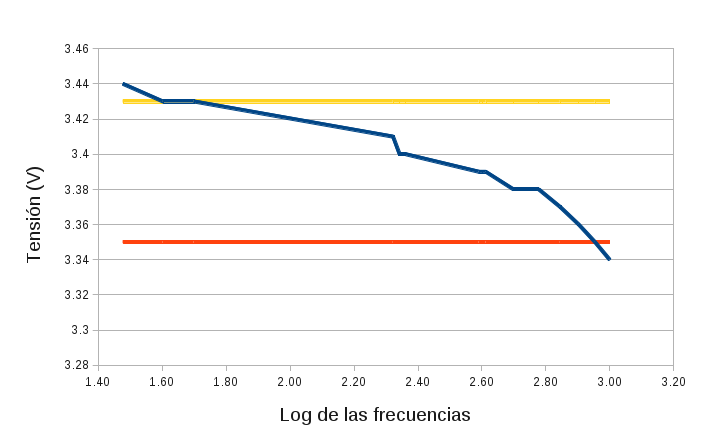
\includegraphics[width=0.80\textwidth]{images/tablaDVM.png}
\caption{Gráfico de los valores medidos con el voltímetro DVM.}
\end{figure}


\subsubsection{Multímetro True-RMS}

La incertidumbre para la escala utilizada es:

\begin{equation}
 	\Delta(V) = 1\%\times V_{medido} + 3d\times 1mV.
\end{equation}
\medskip


\bigskip
\begin{table}[h]
	\begin{center}
	\begin{tabular}{|c|c|c|}\hline
	\textbf{f(Hz)} & \textbf{V(Volts)} & \textbf{$\Delta$V(Volts)} \\ \hline
	80 & 3.417 & 0.037\\ \hline
    90 & 3.418 & 0.037\\ \hline
    100 & 3.419 & 0.037\\ \hline
	110 & 3.423 & 0.037\\ \hline
	440 & 3.419 & 0.037\\ \hline
	450 & 3.420 & 0.037\\ \hline
	460 & 3.420 & 0.037\\ \hline
	990 & 3.393 & 0.037\\ \hline
	1000 & 3.398 & 0.037\\ \hline
	1010& 3.396 & 0.037\\ \hline
	1500 & 3.385 & 0.037\\ \hline
	1700 & 3.379 & 0.037\\ \hline
	\end{tabular}
	\caption{Tabla de los valores medidos con el voltímetro True-RMS}
	\end{center}
\end{table}
\bigskip

\begin{figure}[h]
\centering
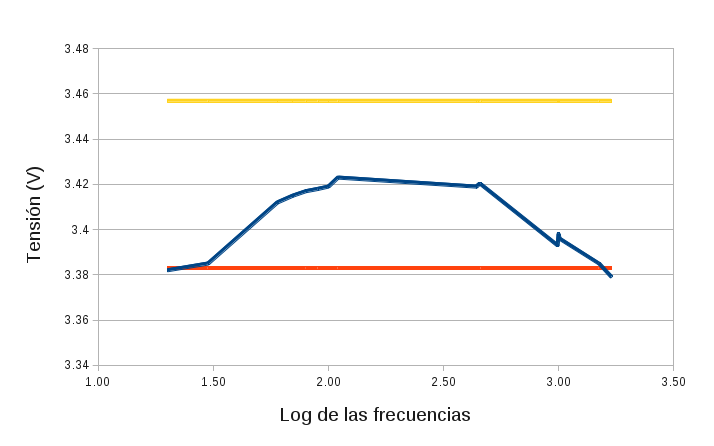
\includegraphics[width=0.80\textwidth]{images/tablaTRUE.png}
\caption{Gráfico de los valores medidos con el voltímetro True-RMS.}
\end{figure}
\bigskip\bigskip\bigskip



Los valores medidos son:

\begin{center}
	$V_{ref} = (3.420 \pm 0.037) V$
\end{center}
\bigskip\bigskip



\subsubsection{Multímetro Analógico}


La incertidumbre para la escala utilizada es:

\begin{equation}
 	\varepsilon_r(V) = 3\%\times V_{medido} + {1 \over 2}\times 0.2V
\end{equation}
\medskip

Valores medidos:

\begin{center}
$V_{ref} = (3.4 \pm 0.2) V$
\end{center}


\newpage
\begin{table}[h]
	\begin{center}
	\begin{tabular}{|c|c|c|}\hline
	\textbf{f(Hz)} & \textbf{V(Volts)} & \textbf{$\Delta$V(Volts)} \\ \hline
	10 & 3.4 & 0.2\\ \hline
    213000 & 3.2 & 0.2\\ \hline
    758000 & 3.0 & 0.2\\ \hline
	\end{tabular}
	\caption{Tabla de los valores obtenidos con el voltímetro analógico}
	\end{center}
\end{table}
\bigskip



	En este cuadro figuran pocos valores, esto es debido a que se tomaron nota de los valores de frecuencia en los que la aguja cambiaba de división. De \textit{10 Hz} para abajo, no se puede especificar el valor medido, ya que la aguja oscila.


\newpage
\begin{figure}[h]
	\centering
	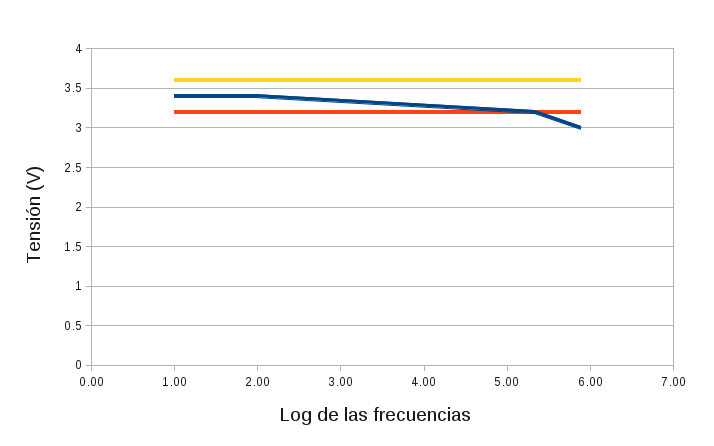
\includegraphics[width=0.80\textwidth]{images/tablaANA.png}
	\caption{Gráfico de los valores medidos con el voltímetro analógico.}
\end{figure}
\bigskip\bigskip



Por lo tanto, los valores aproximados de los anchos de banda son:

\begin{table}[!hbt]
	\begin{center}
	\begin{tabular}{|c|c|}\hline
	\textbf{Voltímetro} & \textbf{Ancho de banda(experimentales)}\\ \hline
    DVM &  $\sim$ (30 - 900)$Hz$\\ \hline
    True - RMS &  $\sim$ (30 - 1500)$Hz$\\ \hline
    Analógico & $\sim$ (10 - 213000)$Hz$\\ \hline
	\end{tabular}
	\caption{Tabla de los anchos de banda experimentales}
	\end{center}
\end{table}
\bigskip




\section{Conclusión}

	De la primera parte se observa que los valores medidos y los valores calculados no diferen mucho, lo que para los multímetros analógico y DVM es notable, ya que multiplcan al valor medio rectificado por el factor de forma de una onda senoidal, y el error resultante no parace ser tan significativo.
	\par
	De la segunda parte resalta el hecho de que los anchos de banda observados en los que son válidas las mediciones realizadas por los instrumentos es en realidad mayor al especificado por el fabricante de estos instrumentos, siendo el analógico el mayor. La diferencia observada en los anchos de banda, debe ser una precaución del fabricante para poder asegurar la fiabilidad del instrumento en los casos más cercanos a los extremos y que la incertidumbre esté dentro de los valores razonables.


% APÉNDICE A

\newpage
\vspace*{4cm}
\begin{center}
	\textbf{\Huge{Apéndice A}} \\
	\bigskip\bigskip
	\Large{\textit{``Cálculos teóricos''}}
\end{center}


\newpage
\section{Cálculos teóricos}
\bigskip

\subsection{Cálculos teóricos en DC}

El valor continuo es el valor medio de la señal:

\begin{center}
\begin{equation}
V_{m} =  {{1}\over{T}} \times \int_{0}^{T} {V(t)} \delta t
\end{equation}
\end{center}
\bigskip

En el caso de la senoidal y de la triangular, al tener un ciclo de trabajo de 50\%, son ondas simétricas, entonces el valor medio es 0.

En el caso de la señal cuadrada:

\begin{center}
\begin{equation}
V =  {5V \times 3ms - 5V \times 7ms \over 10ms }= -2V
\end{equation}
\end{center}
\bigskip


\subsection{Cálculos teóricos en AC}

\subsubsection{Analógico y DVM}

Ambos presentan capacitor, y rectifican a onda completa, calculan el $V_{m_{rect}}$ y muliplcan por el factor de forma que es 1,11.

Onda cuadrada:

\begin{center}
\begin{equation}
V_{ef} = 1,11 \times 2 \times {b \times h \over T} = 1,11 \times 2 \times {7V \times 3ms \over 10ms} = 4,66V
\end{equation}
\end{center}
\medskip


Onda senoidal:

\begin{center}
\begin{equation}
V_{ef} = 1,11 \times {2 \over 2\pi} \times \int_{0}^{\pi} 5V \times \sin (t)\delta t = 3,53 V
\end{equation}
\end{center}
\medskip

Onda triangular:

\begin{center}
\begin{equation}
V_{ef} = 1,11 \times 2 \times {b \times h \over 2 \times T} = 1,11 \times 2 \times {5V \times 
5ms \over 2 \times 10ms} = 2,78V
\end{equation}
\end{center}
\bigskip

\subsubsection{True-RMS}

Presenta un capacitor en la entrada, y realiza el cálculo del valor eficaz:
\begin{center}
\begin{equation}
V_{ef} = \sqrt{ {{1}\over{T}} \times \int_{0}^{T} {V(t)}^2 \delta t}
\end{equation}
\end{center}
\medskip

Onda cuadrada:

\begin{center}
\begin{equation}
V_{ef} = \sqrt{b \times h^2 \over T} = \sqrt{3ms \times (7V)^2 + 7ms \times (3V)^2 \over 10ms} = 4,583V
\end{equation}
\end{center}
\medskip

Onda senoidal:

\begin{center}
\begin{equation}
V_{ef} = \sqrt{{1 \over 2\pi} \times \int_{0}^{2\pi} (5V)^2 \times \sin ^2 (t)\delta t} = 3,536 V
\end{equation}
\end{center}
\medskip

Onda triangular:

\begin{center}
\begin{equation}
V_{ef} = \sqrt{{1\over T}\times 2 \times {b\times h^2 \over 2}} = \sqrt{5ms \times (5V)^2 \over 2 \times 10ms} = 2,500V
\end{equation}
\end{center}
\medskip



% APÉNDICE B

\newpage
\vspace*{4cm}
\begin{center}
	\textbf{\Huge{Apéndice B}} \\
	\bigskip\bigskip
	\Large{\textit{``Hojas de datos de instrumentos de medición''}}
\end{center}

















\end{document}
